
\documentclass[prc,floatfix,superscriptaddress,letter]{revtex4}

\usepackage{color}
\usepackage[normalem]{ulem}
\input epsf

\setlength{\textwidth}{6.5in}
\setlength{\textheight}{9.6in}
\setlength{\oddsidemargin}{0.0in}
\setlength{\topmargin}{-1.0in}
\usepackage{amsmath}
\usepackage{graphicx}
\usepackage{url}
\usepackage{color}
\usepackage{subfigure}
\usepackage{longtable}
\usepackage{dcolumn}



    % See p.105 of "TeX Unbound" for suggested values.
    % See pp. 199-200 of Lamport's "LaTeX" book for details.
    %   General parameters, for ALL pages:
    \renewcommand{\topfraction}{0.9}	% max fraction of floats at top
    \renewcommand{\bottomfraction}{0.8}	% max fraction of floats at bottom
    %   Parameters for TEXT pages (not float pages):
    \setcounter{topnumber}{2}
    \setcounter{bottomnumber}{2}
    \setcounter{totalnumber}{4}     % 2 may work better
    \setcounter{dbltopnumber}{2}    % for 2-column pages
    \renewcommand{\dbltopfraction}{0.9}	% fit big float above 2-col. text
    \renewcommand{\textfraction}{0.07}	% allow minimal text w. figs
    %   Parameters for FLOAT pages (not text pages):
    \renewcommand{\floatpagefraction}{0.7}	% require fuller float pages
	% N.B.: floatpagefraction MUST be less than topfraction !!
    \renewcommand{\dblfloatpagefraction}{0.7}	% require fuller float pages
    
    \newcommand{\jpsi}{$J/\psi$ }
\begin{document}


\title{Review of the CLAS12 Analysis Proposal "Hexaquarks at CLAS12"  \\
by M. Bashkanov, D.P. Watts and  N. Zachariou (the York group)}
\author{Valery Kubarovsky and Zhiwen Zhao}
\date{\today}
\maketitle

The suggested CLAS12 analysis proposal is devoted to the study of the extremely interesting topic. It was suggested to search for the heavy strange partners of the $d^*(2380)$ particle that has possible interpretation as a hexaquark state. This resonance was seen in the $d\pi^0\pi^0$, $d\pi^+\pi^-$ and $pp\pi^0\pi^-$ channels in the hadro- and photo-production experiments. The York group suggested the measurements that will allow the discovery of all  $d^*(2380)$ multiplet members in the case if $d^*$ belongs to the SU(3) antidecuplet. This is very challenging task and this statement is too strong in our view. But there is no doubts that the goal of the proposed study is at the cutting edge of the particle spectroscopy. The group is going on to study hexaquark candidates with strangeness zero, one, two and three using the run group B data set.

We can only suggest that Fig. 5 reflects the MC study of the CLAS12 detector. The information provided in the proposal is very limited and it is very weak side of this paper.  We need more information how these pictures were generated and how the acceptance was calculated.
Does this picture show the ability of CLAS12 to detect $d^*(2380)$ in the $d\pi^0\pi^0$ decay mode?
If so, we can say that the acceptance near the resonance mass is very low and 
is fast changing in this mass region.
 It will be very desirable to have at least the rough estimation of the $d^*$ expected statistics from rg-B data set.


The group presented some preliminary search of $d_s$ based on the CLAS6 g13 data, attempting to study 
$d_s\to \Sigma^*\Delta$ decay mode. It is very good. However, there was no attempt to use the existing rg-B data set 
to demonstrate the CLAS12 ability to search for this resonance. The current status of the rg-B analysis software is giving such a possibility. It is important or even necessary step in the submitting the analysis project that will determine the 
 research activity of  several PhD students.

It was not clear for us   why the charged kaon channel 
is less promising than neutral kaon channel for the d$_s$ production.


We can only guess that Fig.~10 presents the simulation of the CLAS12 detector. Please provide the full description of the picture that you have presented! What kind of generator did you use for the MC simulation?
Do you have estimation of the $d_s$ mass? 
There is one big factor that is missing in the calculations. We know that the track reconstruction efficiency
is not 100\% in CLAS12. At the rg-B luminosity the track reconstruction efficiency is around 80\%.
If you are going to detect 7 particles (see Fig. 10) you will have additional factor $0.8^7=0.2$. 
It means that the expected number of events will be 5 times less than calculated using acceptance presented in the picture.

What is the model that you are using to calculate background presented in Fig. 13?
It was written in the capture that blue line with a maximum near 1760 MeV represents $d_{ss}$. Is it really so?

We have the same questions and remarks for the Fig. 15 as we have for the Fig. 10.

The weak point of this proposal is absent of the preliminary study of the  reactions with one, two and three kaons in the final state. It may show how clean these reactions are. In addition, we can   estimate the statistics that
 we have in run group B. Some rg-A data analysis was presented recently from the York group.
 Please take a look at the Fig. \ref{fig:e-K+_mm} and \ref{fig:e-K+K+_mm}. The situation is not very promising as for now.
 Even with one detected kaon the missing mass contains a significant background.
 The missing mass in the reaction $ep\to e'K^+K^+X$ does not show any signal from $\Xi$ baryon at all.
 There is significant background below the $\Xi$ mass. The figure 18 (is it rg-A data by the way?) presents only background events. One of the reasons of the significant background in these reactions is kaon particle identification.
 Taking into account that any kaon brings a factor of 10 in comparison with pion   
 we can estimate that $K^+K^-K^+$ production will be suppressed by a factor of 1000 in comparison with $\pi^+\pi^+\pi^+$.
 It means that the suppression of the pion background has to be done at the level at least $10^{-3}-10^{-4}$ that is extremely difficult.
 It is our guess that the situation will be even worse with the deuterium target. In our view it is very important to provide similar preliminary analysis of the rg-B data in advance.
 

We have also several editorial remarks. \begin{enumerate}

\item The references are not in order. Many references are just absent, see for example  Fig. 2 capture and on page 14.
\item Reference 5 is incomplete, there is no date in it.
\item There is no reference to Fig. 9.
\item Page 14. No reference provided:  It was shown already in
Ref. ???? that a $\Omega \pi$  contact term is very repulsive.
\item Page 14. Reference absent:First evaluation were preformed based on CLAS12 data runs() ????
\item Please put dot at the end of each reference in the paper.
\end{enumerate}


In general, we conclude that  this is very interesting and important topic to 
study, but it's hard for us to judge how promising it is with the 
information provided. 

\begin{figure}
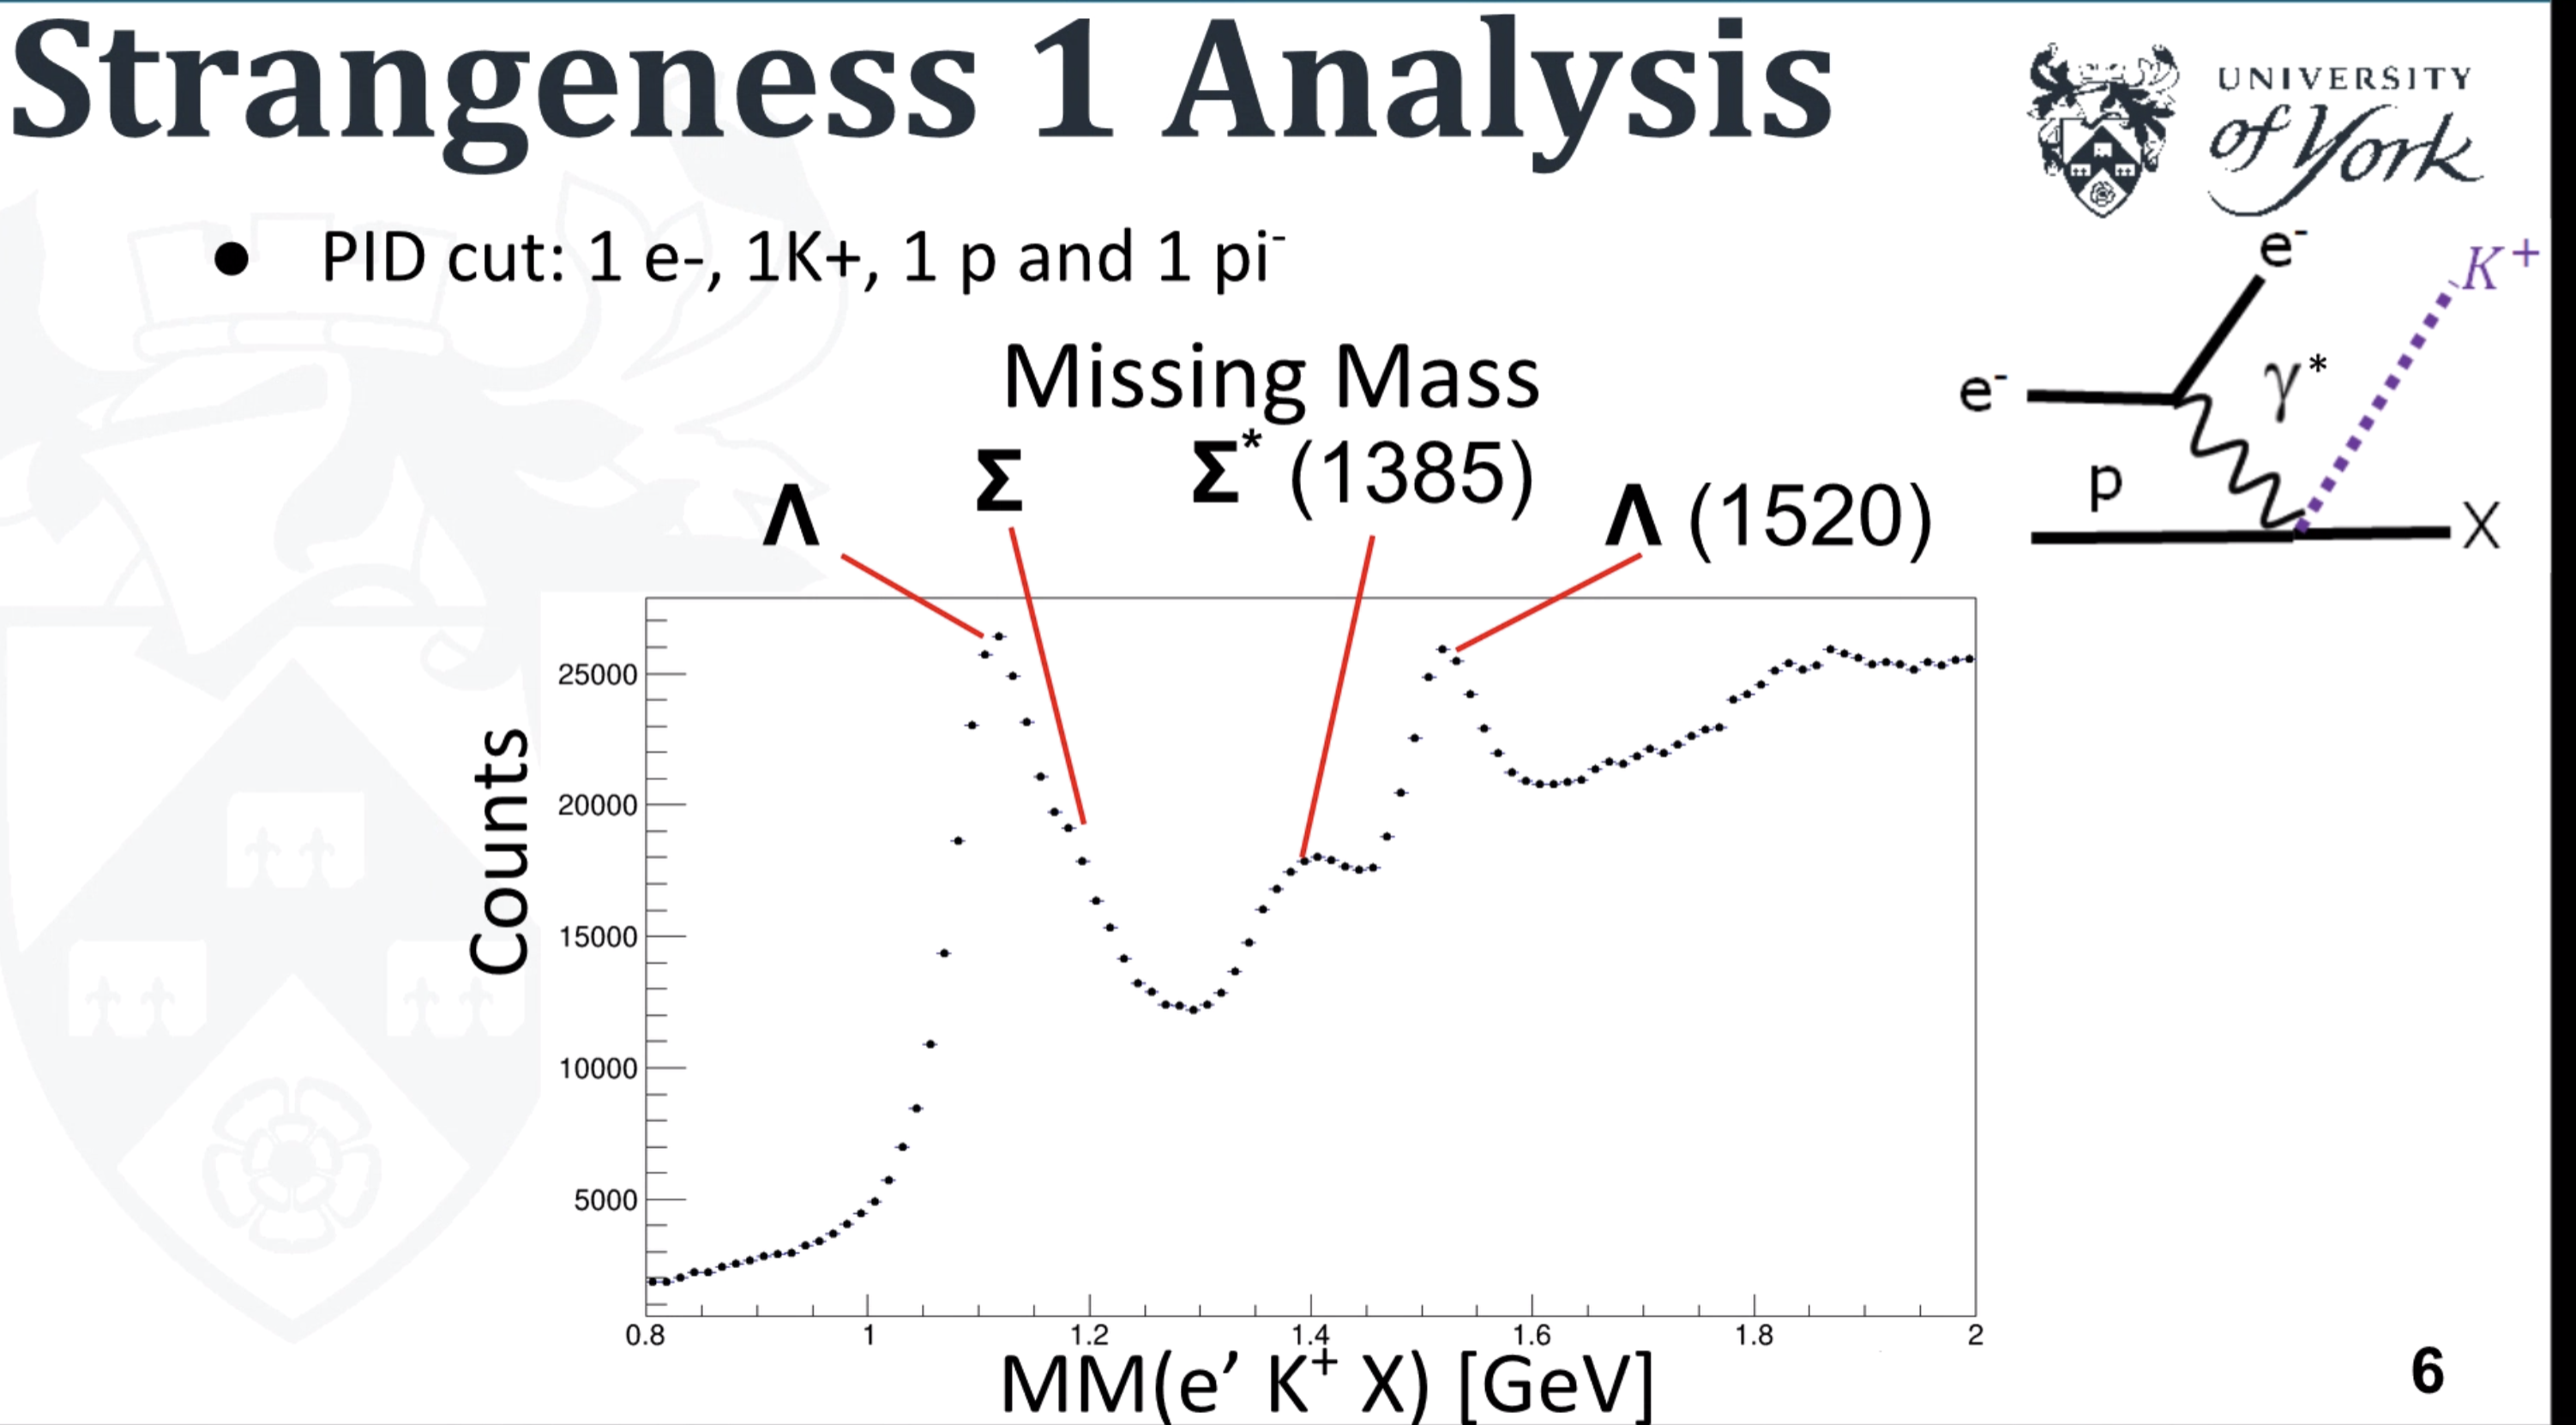
\includegraphics[width=10cm]{e-K+_mm.png} 
\caption{
Missing mass in the reaction $ep\to e'p'K^+X$, RG-A data set.
} 
\label{fig:e-K+_mm}
\end{figure}
 
\begin{figure}
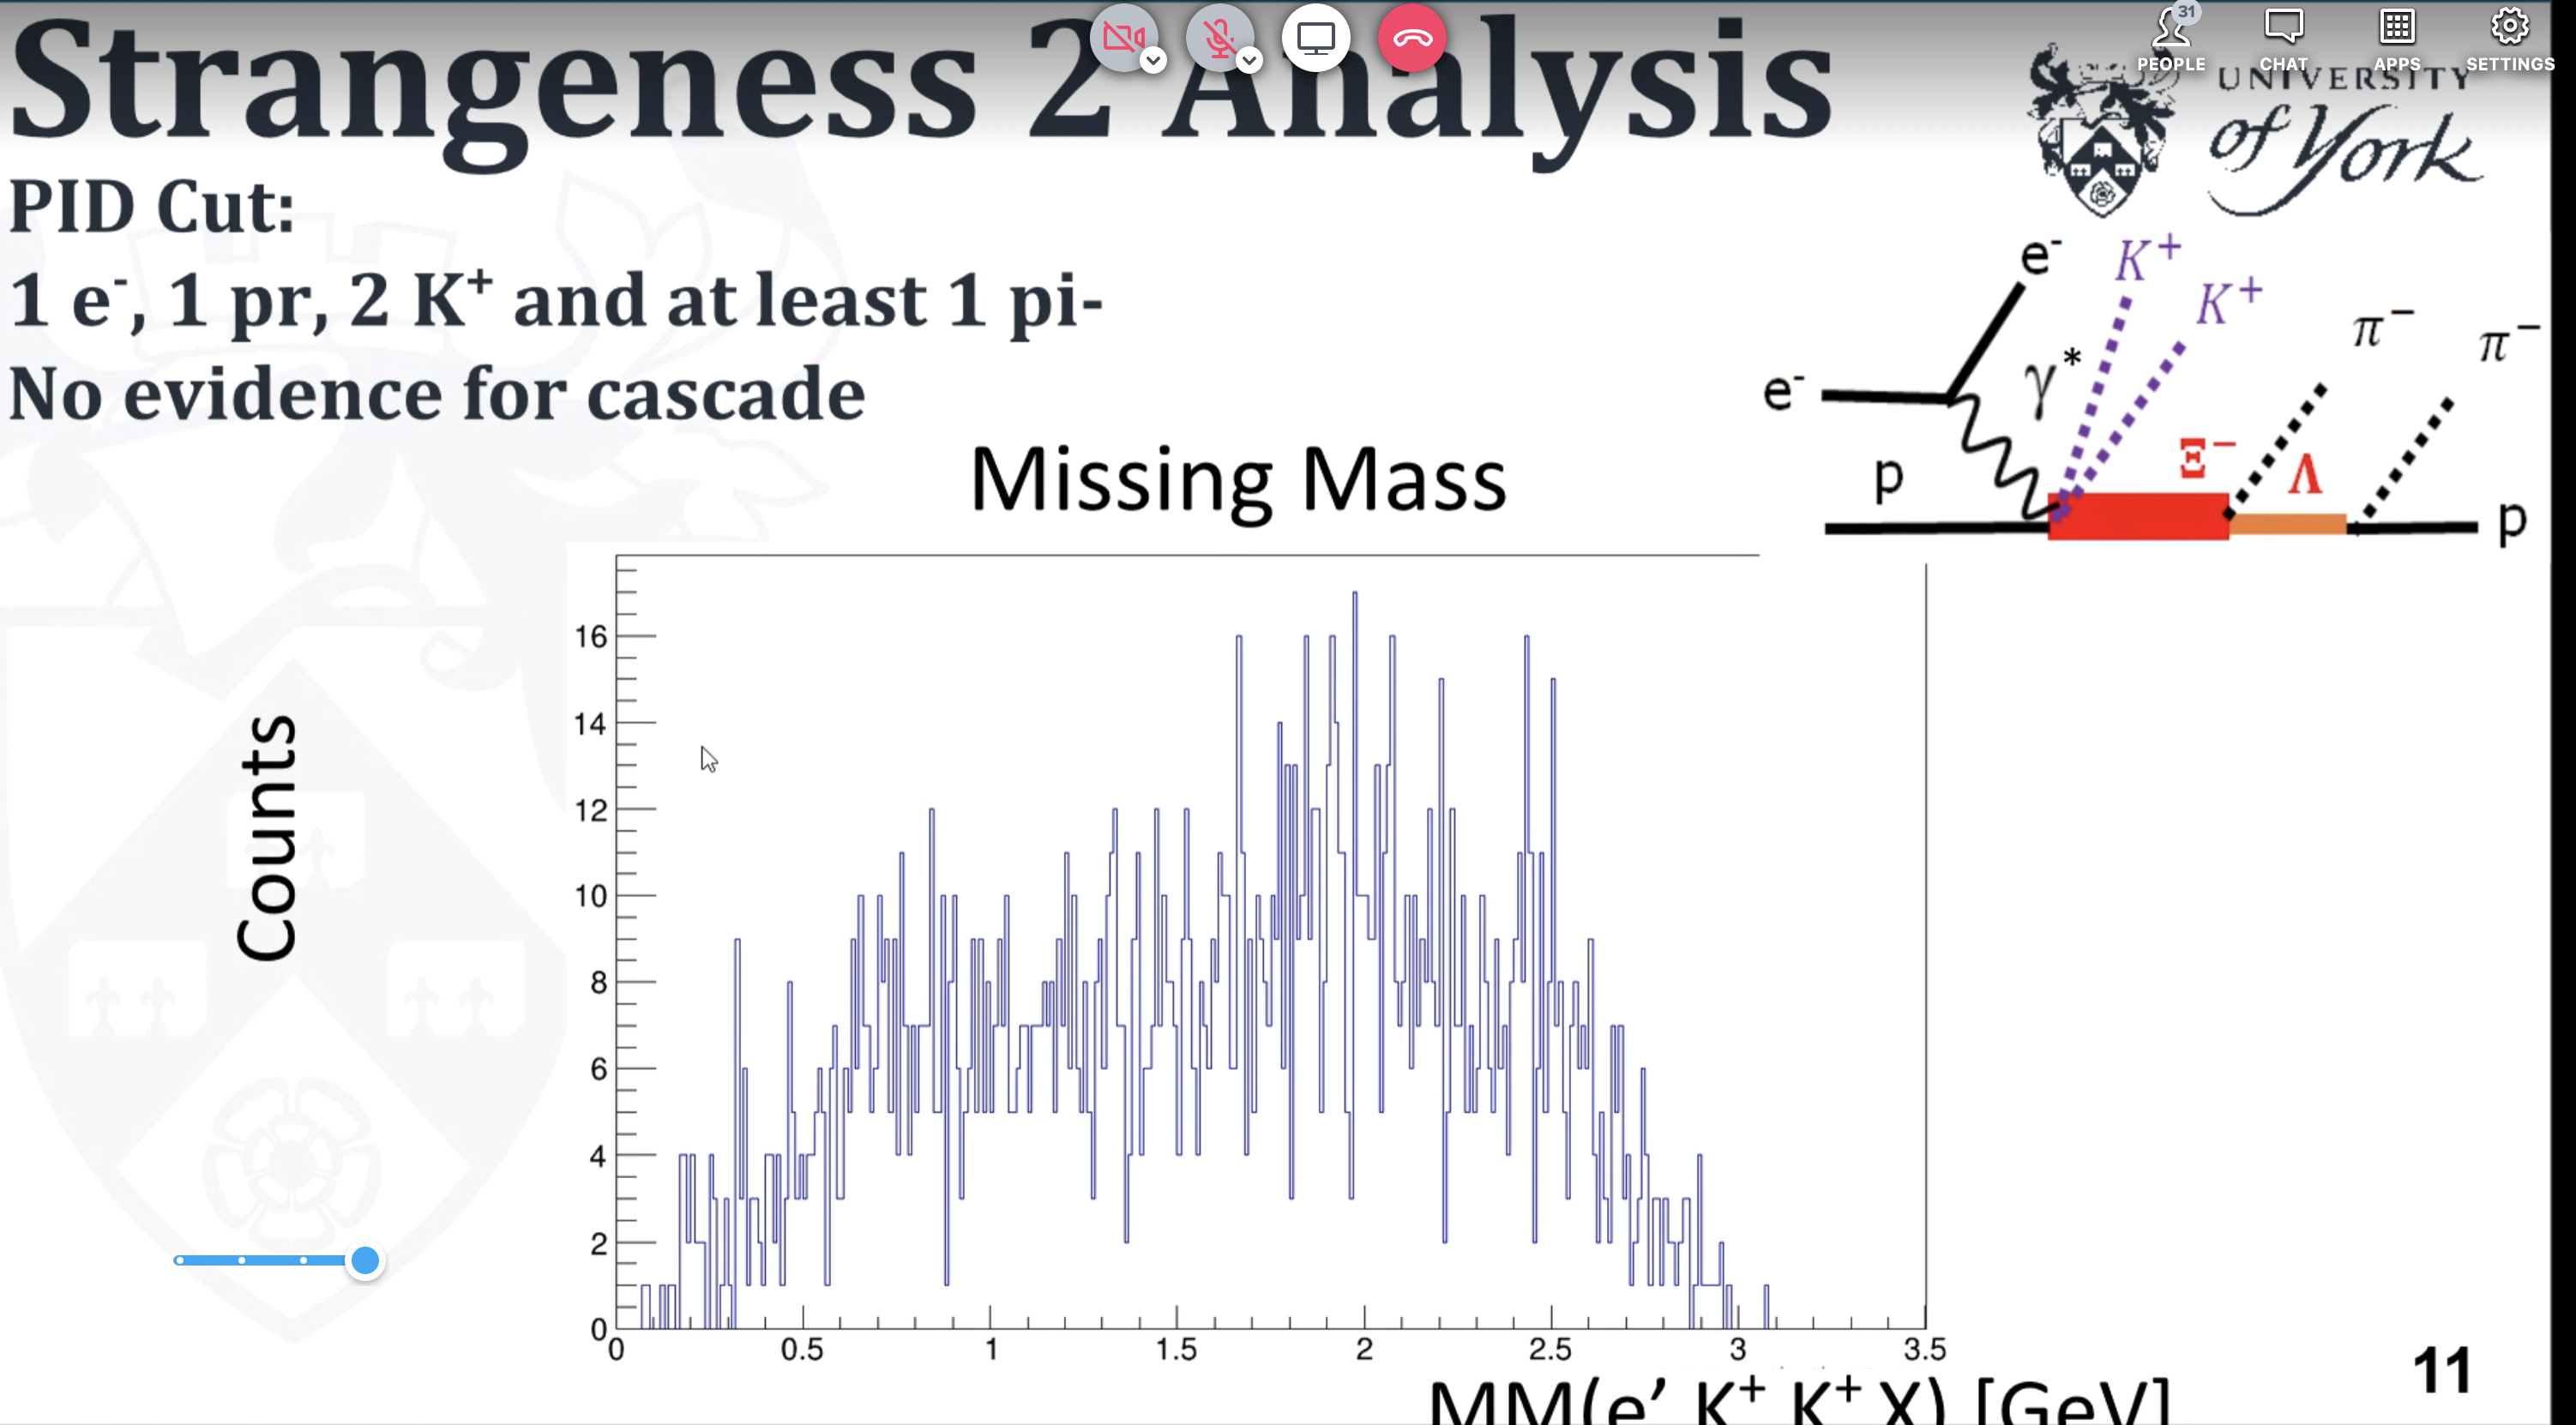
\includegraphics[width=10cm]{e-K+K+_mm.png} 
\caption{
Missing mass in the reaction $ep\to e'p'K^+K^+X$, RG-A data set.
} 
\label{fig:e-K+K+_mm}
\end{figure}





\end{document}